\pdfoutput=1
\documentclass[11pt]{article}
\usepackage[margin=1in]{geometry}
\usepackage{amsmath,amssymb,amsthm}
\usepackage{enumitem}
\usepackage{booktabs}
\usepackage{longtable}
\usepackage{array}
\usepackage{tikz}
\usetikzlibrary{arrows.meta,positioning}
\usepackage{hyperref}
\hypersetup{hidelinks,
  pdftitle={Forgetting and completeness: the centre of the passage from Theorem 3.11 to Corollary 3.12 in inter-universal Teichmueller theory},
  pdfauthor={Toshihisa Urahigashi}}

\theoremstyle{plain}
\newtheorem{theorem}{Theorem}[section]
\newtheorem{proposition}[theorem]{Proposition}
\theoremstyle{definition}
\newtheorem{definition}[theorem]{Definition}
\theoremstyle{remark}
\newtheorem{remark}[theorem]{Remark}

\newcommand{\FRAME}{\textup{[FRAME]}}
\newcommand{\EST}{\textup{[EST]}}
\newcommand{\OPEN}{\textup{[OPEN]}}
\newcommand{\Hmark}{\textup{[H]}}
\newcommand{\vol}{\operatorname{vol}}
\newcommand{\procVol}{\operatorname{procVol}}
\newcommand{\linkScale}{\operatorname{linkScale}}
\newcommand{\cO}{\mathcal O}

\title{Forgetting and completeness: the centre of the passage\\
from Theorem~3.11 to Corollary~3.12\\
in inter-universal Teichm\"uller theory}
\author{Toshihisa Urahigashi\\
\small\texttt{123026.urahigashi.toshihisa@gmail.com}}
\date{Version 1.1.1 --- 11 November 2026\\[3pt]
\small Independent researcher. This work was carried out personally and is
unrelated to any institutional affiliation.\\[3pt]
\small ORCID \href{https://orcid.org/0009-0004-0460-6242}{\texttt{0009-0004-0460-6242}}\\[-2pt]
\small \href{https://doi.org/10.5281/zenodo.24135926}{doi:10.5281/zenodo.24135926} (all versions: \href{https://doi.org/10.5281/zenodo.24135420}{10.5281/zenodo.24135420})}

\begin{document}
\maketitle

\begin{abstract}
We formulate the passage from Theorem~3.11 to Corollary~3.12 in
inter-universal Teichm\"uller theory (IUT) as a problem of
\emph{completeness} in the sense of abstract interpretation.  A
forgetful map $\alpha:X\to A$ is complete for a query $Q:X\to Y$ if
$Q$ factors through $\alpha$, that is, if the abstract data determine
the answer to $Q$.  The same forgetting can be complete for one query
and incomplete for another: sign abstraction is complete for the sign
of a product but not for the sign of a sum, and interval abstraction
drops the correlation between two uses of the same datum.
Completeness is therefore a relation between an abstraction and a
query, and local completeness at each interface does not in general
compose.

We first state, in a form checked in Lean, the criterion for
completeness, its restoration by a tracked invariant, and the
sufficiency and---on extremal data with no slack---the sharpness of
scale preservation.  We then read the multiradial machinery as one
diagram: a tower of forgettings from initial $\Theta$-data through
fundamental groups, mono-theta environments, prime-strips, unit and
value-group parts and realified Frobenioids down to log-volume,
together with the reverse mono-analytic reconstruction flow and the
horizontal $\mathfrak{log}$-link and $\Theta$-link.  In the cited
theory $T$ that fixes the log-volume content cited in the proof of
Corollary~3.12, the Corollary~3.12-shaped conclusion does not follow
from $T$ alone, and it does follow once the scale defect
$\Delta=(s-1)\vol(\theta)$ satisfies $\Delta\le 0$; preservation
itself is the vanishing $\Delta=0$, that is, $s=1$ when
$\vol(\theta)\ne0$.  On extremal data with no slack the conclusion is
equivalent to $\Delta\le0$.  Relative to this route, therefore, a
sufficient condition for the ABC-type conclusion reduces to the
non-trivial completeness problem of whether the real scale is
preserved through the whole transport, which contains forgetful
steps.  This is not an unconditional equivalence with the ABC
conjecture itself.

An audit of the relevant interfaces in IUT~I--IV and in
\cite{FrdI,EtTh,AbsTopIII} finds each of them locally closed: Tate
parameter reconstruction, cyclotomic synchronization, the discrete
valuation step, unit-side indeterminacy, within-copy volume
normalization, and the three-tier classification of degrees under
realification.  What remains is a single square: whether the actual
construction supplies a lift of the $\Theta$-link, given between bare
prime-strips, to marked prime-strips preserving generators and scale.
The reduction also shrinks the formalization target: what has to be
formalized is not all of IUT, but only the interfaces needed to
decide the sign of $\Delta$.  This paper decides neither
Corollary~3.12 nor the ABC conjecture.
\end{abstract}

\noindent\textbf{Keywords:} inter-universal Teichm\"uller theory,
Corollary~3.12, abstract interpretation, completeness, forgetful
functor, dependency problem, realification, scale, Lean.

\medskip
\noindent Marks used below: \FRAME{} framing or translation;
\EST{} proved here or verified in the source; \OPEN{} unresolved;
\Hmark{} the present author's reading or interpretation.

\section{Introduction: two questions}

The dispute over Mochizuki's inter-universal Teichm\"uller theory is
often discussed as a single question.  At least the following two
must be separated.

\begin{description}[style=nextline]
\item[Question S (specification).] Does the conclusion of
Corollary~3.12 follow from the explicitly stated log-volume content
of the results cited in its proof alone?
\item[Question C (construction).] Does the actual construction of
IUT preserve, from end to end, the correlations (initial data,
labels, choices of roots, real scale) that are not recorded in the
summaries of the cited properties?
\end{description}

\EST{} The preceding study \cite{U26} showed, by countermodels
checked in Lean, that the answer to Question~S is no for the theory
obtained by fixing the cited range, and that a weak form of the
conclusion does follow.  The present paper does not repeat that
result.  Its purpose is to state precisely, in the language of
forgetting and completeness, where the gap lives and what would have
to be extracted to make Question~C decidable.

\FRAME{} The central reading of this paper is the following.  The
multiradial machinery consists of a sequence of forgetful steps,
each discarding information stage by stage, together with a reverse
flow of mono-analytic reconstructions that recover discarded
structure.  At each interface one can ask for which queries the
answer is not lost.  The query of Corollary~3.12 is not a local
query at a single interface; it is a correlation query that runs
across the same initial data and the shared markings.  Hence each
interface may be locally exact while the composite is incomplete for
that query.

\Hmark{} This reading is consistent with Mochizuki's own
exposition.  The source repeatedly states that distinct arithmetic
holomorphic structures are not to be confused, that they are related
only through the shared shadow of prime-strips, and that the
cyclotome and the value-group part are shielded from unit-side
indeterminacy.  In the language of this paper, this is the claim
that the construction is designed to track the labels.  The point at
issue is whether that claim is closed as a proof at the level of the
cited statements.

In this paper the remaining point is called the \emph{centre}
(Japanese: \emph{honmaru}, the innermost keep of a castle), not a
wall.  Seen from the specification side it appears as a wall that
the cited properties alone cannot cross.  Once it has been isolated
as a completeness problem, it appears instead as the central
proposition that remains to be proved; if that completeness holds,
this route reaches the ABC conjecture.  ``Centre'' is thus the name
of the single point where the remaining work is concentrated, with
no connotation of unattainability.

\section{Simple examples first: when it is preserved and when it breaks}

\subsection{Forgetting signs: preserved for products, broken for sums}

Consider the forgetful map $\operatorname{sign}:\mathbb
Z\to\{-1,0,1\}$ that keeps only the sign of an integer, and the
abstraction $\alpha(a,b)=(\operatorname{sign}a,\operatorname{sign}b)$
of a pair of integers.  For one and the same $\alpha$, completeness
is opposite for the two queries:

\begin{center}
\begin{tabular}{lll}
\toprule
Query & Result & Reason / witness\\
\midrule
Is $\operatorname{sign}(ab)$ determined? & complete &
$\operatorname{sign}(ab)=\operatorname{sign}(a)\operatorname{sign}(b)$\\
Is $\operatorname{sign}(a+b)$ determined? & incomplete &
$(1,-1)$ and $(2,-1)$ share the image $(+,-)$\\
&& but the signs of the sums are $0$ and $+$\\
\bottomrule
\end{tabular}
\end{center}

\EST{} This contrast is checked in Lean as
\texttt{completeFor\_sign\_mul} and \texttt{not\_completeFor\_sign\_add}.
The same sign contrast (complete for multiplication, incomplete for
addition) is also the introductory example of \cite{GRS00}.  What
this shows is that completeness is not a property of an abstraction
alone but a relation between an abstraction and a query.  A
forgetting that keeps multiplicative structure may be complete for
multiplicative queries and incomplete for queries involving
addition.  This is the smallest model for reading the steps of IUT
in which addition is forgotten in the passage to prime-strips.

\subsection{Interval arithmetic: forget the correlation and even
$x-x$ is undetermined}

Suppose a number $x$ is known only to lie in the interval $[0,1]$.
Summarizing componentwise by intervals, the two uses $(x,x)$ of the
same $x$ become $([0,1],[0,1])$, and the difference spreads to
$[-1,1]$.  From the abstract image alone one cannot distinguish the
pair $(0,0)$ (difference $0$) from the pair $(0,1)$ (difference
$-1$).  This is the classical \emph{dependency problem}
\cite{Moore} (for a modern textbook treatment see \cite{MKC09}).

The cure is also classical.  Attach a shared label to each
occurrence---the noise symbols of affine arithmetic---so that the
information ``the two copies are the same datum'' is carried along;
then at least whether the difference is zero is decided again
\cite{FigStolfi}.  The point is that even if every local interval
computation is exact, the end-to-end correlation query becomes
incomplete at the moment the shared label is dropped.

\begin{remark}[The pattern used repeatedly below]
Local completeness fails to compose not because a computation is
wrong, but because an interface summary does not record the
correlation ``the same thing was used twice''.  Restoration requires
not a finer abstraction but carrying along an invariant that
represents the lost correlation.
\end{remark}

\Hmark{} In IUT, the counterparts of the shared label are the
relativity to initial $\Theta$-data, the $\mathrm{LabCusp}$ labels,
the choices of roots and theta values, and finally the relative
scale at realification.  The question of this paper is whether the
last of these, the scale, is preserved through an actual run.

\section{The frame, stated rigorously}

Abstract interpretation is the theory that organizes approximate
computation by Galois insertions and abstract domains
\cite{CC77,CC79}, and completeness has been studied there as the
property that abstract computations accumulate no loss of
information relative to concrete computations \cite{GR97,GRS00}.
Here we use neither the order structure nor fixpoints; we extract
only the minimal factorization form that is needed.  This is a
deliberate simplification, and the statements of this paper are
claimed only inside the simplified frame.

\begin{definition}[Completeness]\label{def:complete}
For maps $\alpha:X\to A$ and $Q:X\to Y$, we say that $\alpha$ is
\emph{complete for} $Q$ if there exists $\widehat Q:A\to Y$ with
$Q=\widehat Q\circ\alpha$.  In Lean this is \texttt{CompleteFor}.
\end{definition}

\begin{proposition}[Fibre criterion]\label{prop:fibre}\EST{}
If $\alpha$ is complete for $Q$, then $\alpha(x_1)=\alpha(x_2)$
implies $Q(x_1)=Q(x_2)$.  Conversely, if $Y$ is nonempty and $Q$ is
constant on every fibre of $\alpha$, then $\alpha$ is complete for
$Q$.  Hence incompleteness is always witnessed by two states with
the same abstract image and different answers.
\end{proposition}

\begin{proposition}[Restoration by a tracked invariant]\EST{}
If $Q$ factors through $x\mapsto(\alpha(x),c(x))$ and the invariant
$c$ is normalized to a constant $c_0$ on the states under
consideration, then on those states $\alpha(x_1)=\alpha(x_2)$ implies
$Q(x_1)=Q(x_2)$.  In Lean, \texttt{complete\_on\_normalized} is
proved without axioms.
\end{proposition}

\begin{proposition}[Reduction theorem: the scale defect]\label{prop:defect}\EST{}
For the signed log-volume relation $\vol(q)=s\cdot\vol(\theta)$, put
$\Delta=(s-1)\vol(\theta)$.  Then:
\begin{enumerate}[label=\textup{(\roman*)}]
\item (Sufficiency) If $\vol(\theta)\le\vol(H)$ and $\Delta\le0$,
then $\vol(q)\le\vol(H)$.
\item (Equivalence with slack) $\vol(q)\le\vol(H)$ if and only if
$\Delta\le\vol(H)-\vol(\theta)$.  In particular, with no slack it is
equivalent to $\Delta\le0$.
\item (Preservation itself) If $\vol(\theta)\ne0$, then $\Delta=0$
if and only if $s=1$.
\item (Sign translation) In the convention of \cite{U26}, where the
relevant log-volumes are negative, $\Delta\le0$ is equivalent to
$s\ge1$, and the countermodel lies on the side $s=3/14<1$.
\end{enumerate}
In Lean these are
\texttt{conclusion\_of\_nonpositive\_scale\_defect},
\texttt{conclusion\_iff\_defect\_le\_slack},
\texttt{scale\_defect\_eq\_zero\_iff\_scale\_eq\_one} and
\texttt{nonpositive\_defect\_iff\_one\_le\_of\_neg}.
\end{proposition}

The direction of a one-sided inequality depends on the
parameterization (in the convention where a multiplier $t$ acts on a
nonnegative hull bound, the favourable side is $t\le1$).  We
therefore take the convention-independent defect $\Delta$ as the
main actor, and define preservation itself as $\Delta=0$, i.e.\ $s=1$.

\begin{center}
\begin{tabular}{llll}
\toprule
Convention & Favourable side & Preservation & Countermodel\\
\midrule
\cite{U26}: $\vol(q)=s\vol(\theta)$, & $s\ge1$ & $s=1$ &
$s=3/14<1$ fails\\
\quad log-volumes negative & ($\Delta\le0$) & ($\Delta=0$) &\\
Hull bound: $q_{\mathrm{vol}}\le t\,h_{\mathrm{vol}}$, & $t\le1$ &
$t=1$ & reciprocal\\ \quad nonnegative & &
& parameterization\\
\bottomrule
\end{tabular}
\end{center}

\FRAME{} Propositions~3.3 and \ref{prop:defect} are elementary; they
are not deep theorems by themselves.  Their role is to fix the
logical shape of the claim: a failure of completeness is turned into
the checkable question ``which invariant is not being tracked?'',
and the additional principle needed for restoration can be named as
a single item.  The mathematical difficulty is thereby transferred
to whether that additional principle is supplied by the actual
construction.

\Hmark{} Reading an $\alpha$ off a text is itself not a theorem.
What can be guaranteed here is the implication ``complete for the
stated $\alpha$'', together with the auditability of where each
component of that $\alpha$ comes from in the source.  Formalization
does not remove this interpretive boundary; it concentrates it into
one visible point.

\section{Reading IUT as a diagram of forgettings}

\FRAME{} Read the multiradial machinery as the following tower of
stages: from full arithmetic data, through tempered fundamental
groups and mono-theta environments, prime-strips, unit parts and
value-group parts, and realified Frobenioids, down finally to the
real number given by log-volume.  Each stage forgets part of the
structure.  In the reverse direction, mono-analytic reconstruction
recovers part of what was dropped.  Horizontally there are the
$\mathfrak{log}$-link inside a column, the $\Theta$-link between
columns, and the Kummer correspondences and evaluation maps.
Appendix~A collects the whole picture in one figure.

\begin{figure}[h]
\centering
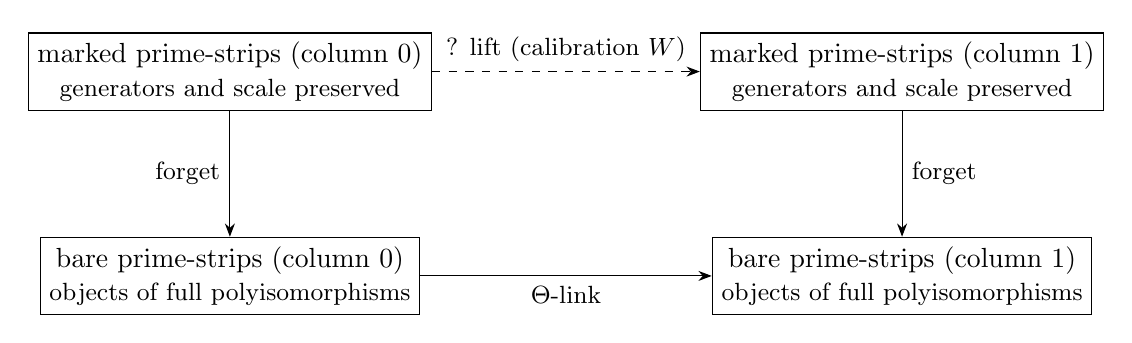
\begin{tikzpicture}[>=Stealth, node distance=2.2cm]
\node[draw, align=center] (m0) {marked prime-strips (column 0)\\
\small generators and scale preserved};
\node[draw, align=center, right=3.4cm of m0] (m1)
{marked prime-strips (column 1)\\
\small generators and scale preserved};
\node[draw, align=center, below=1.6cm of m0] (b0)
{bare prime-strips (column 0)\\
\small objects of full polyisomorphisms};
\node[draw, align=center, below=1.6cm of m1] (b1)
{bare prime-strips (column 1)\\
\small objects of full polyisomorphisms};
\draw[->, dashed] (m0) -- node[above]{\small ? lift (calibration $W$)} (m1);
\draw[->] (m0) -- node[left]{\small forget} (b0);
\draw[->] (m1) -- node[right]{\small forget} (b1);
\draw[->] (b0) -- node[below]{\small $\Theta$-link} (b1);
\end{tikzpicture}
\caption{The missing square.  The lower arrow exists as a full
polyisomorphism in the sense of \cite[Def.~3.8(ii)]{IUT3}.  The
question is whether the actual construction supplies the upper
arrow preserving the same initial-data calibration.}
\label{fig:square}
\end{figure}

That the lower arrow exists and that the upper arrow exists are
different assertions.  From the lower arrow alone there remains the
relative scale $c$, the ratio of the readouts in the two columns.
Transported once around a loop, $c$ may be regarded as the holonomy
of the loop; $c=1$ is the condition that the cocycle is a
coboundary, i.e.\ that there is a marking making every transport
have scale $1$.  Since the scale of each copy is anchored
absolutely, e.g.\ by $\mu_k(\cO_k)=1$, the number $c$ is not a mere
freedom of convention but an invariant of the chosen member.

\FRAME{} In categorical language this is a lifting problem for a
forgetful functor $U:\mathbf{Marked}\to\mathbf{Bare}$.  A
multiradial representation may be read as a functorial assignment
from the log-theta-lattice to containers, and the question of
Corollary~3.12 asks whether that assignment preserves one specific
diagram, the comparison between columns.  Category theory provides
no magic proof here; it provides a language in which the squares to
be checked can be listed finitely and the faces that are already
closed can be separated from the one that is open.

\section{Relative reduction to scale preservation: what is and is
not equivalent}

We separate the ranges in which the often-quoted phrase ``an
equivalent reformulation of a sufficient condition for ABC'' is
accurate.  The claim made in this paper is the following relative
reduction.  In the cited theory $T$, which fixes the log-volume
content cited in the proof of Corollary~3.12, and in the models
formalized in that range:
\begin{enumerate}[label=\textup{(\arabic*)}]
\item from $T$ alone the strong, Corollary~3.12-shaped conclusion
does not follow;
\item if the scale-defect condition $\Delta\le0$ (preservation
itself being $\Delta=0$, i.e.\ $s=1$) is added to $T$, the strong
conclusion does follow (Proposition~\ref{prop:defect});
\item on extremal data with no slack the conclusion is equivalent
to $\Delta\le0$; hence for uniform derivations the scale condition
is not only sufficient but sharp.
\end{enumerate}
In this sense, relative to this route of IUT---from Theorem~3.11
through Corollary~3.12 to the numerical assembly of IUT~IV, as
assembled in the source---a sufficient condition for the ABC-type
conclusion reduces to the completeness problem of whether the real
scale is preserved through the whole transport, which contains
forgetful steps.  That is, this scale-preservation problem is a
sufficient condition for ABC, and IUT, along this route, reduces ABC
to it.  Is that preservation then solved, proved, refuted, or
verified?  The answer is no in every case (\S\S6--7).

What is \emph{not} claimed is an unconditional equivalence between
the ABC conjecture itself and this completeness problem.  For an
individual elliptic curve the height inequality may hold for reasons
of slack or by a different proof route, in which case $\Delta\le0$
is not necessary.  Equivalence holds only relative to the fixed
cited theory and uniform derivations, or on extremal data.

\EST{} Proposition~26 of \cite{U26} contains the nucleus of this
reduction: (a) the gap is not bridged inside the container alone;
(b) identifying the two pilots yields the conclusion and $s=1$;
(c) from $s=1$ and nonzero measure the conclusion follows, so that
contrapositively a failure of the conclusion forces $s\ne1$.  The
general factorization shape through the pair $(\alpha,s)$ is not a
numbered proposition there, which is why it is presented separately
here as Propositions~3.3 and \ref{prop:defect}.

\EST{} In the sideways Lean formalization as well, the gap to the
conclusion is bounded by the defect
$\Delta=(\linkScale-1)\cdot\procVol(\theta)$; the
Corollary~3.12 shape is its $\Delta\le0$ point and preservation
itself is the $\Delta=0$ point.  The same ``defect $\le$ slack''
shape has been obtained in the repository of Project LANA, where
Step~(xi) is shown to be equivalent to adding the inequality
$(s^{-1}-1)a\le V$ to a Theorem~3.11-level package (\texttt{xi\_iff})
\cite{lana}; this is the reciprocal parameterization of
Proposition~\ref{prop:defect}(ii).  The equality (9-1) of
\cite[\S9.2]{LANA} states the same content from the equality side,
as commutativity of a diagram.  The contribution of the present
paper is therefore not the discovery of this reduction itself, but
its restatement in the language of completeness and the
localization of what remains by an interface-by-interface audit.
Within that audited decomposition, end-to-end completeness reduces
to the liftability in the missing square.  This is a reduction
relative to the audited decomposition in which the other faces are
closed; it is not an unconditional equivalence theorem about the
whole construction.

\section{The interface-by-interface audit}

The following table summarizes the author's audit and formalization
of the interfaces in IUT~I--IV and \cite{FrdI,EtTh,AbsTopIII},
carried out against checked editions of the sources.  ``Closed''
means that completeness for the local query at that interface was
verified as a statement of the source or as a Lean theorem; it does
not mean end-to-end completeness.

\begin{center}
\small
\begin{longtable}{>{\raggedright\arraybackslash}p{2.9cm}>{\raggedright\arraybackslash}p{2.0cm}>{\raggedright\arraybackslash}p{1.9cm}>{\raggedright\arraybackslash}p{6.2cm}}
\toprule
Interface & Kind & Status & Grounds\\
\midrule
\endhead
Identification of initial $\Theta$-data & provenance & fixed by
definition & A provenance condition on both theaters; not a
condition on the choice of member \cite[Def.~3.8(ii)]{IUT3}.\\
Curve to Tate parameter & reconstruction & closed & Intrinsic via
$j$; Lean Tate reconstruction and the identification with
$\log\lVert j(W)\rVert$.\\
Cyclotomic synchronization & reconstruction & closed &
\cite[Cor.~2.19(i)]{EtTh}: finite-level Tate-twist identification;
discrete ambiguity excluded.\\
Local monoid reconstruction & reconstruction & closed &
\cite[Prop.~3.2]{AbsTopIII}: normalization by the unramified
value-monoid generator; rigidity of the value monoid $\mathbb N$.\\
Unit-side indeterminacy & quotient & closed at readout & Ism acts
by a unit scalar; the Galois part preserves at $e=1$ and has only a
displacement bound for $e>1$.\\
Identification at realification & quotient & tiered & The
three-tier $\mathbb R_{>0}/\mathbb Q_{>0}/1$ classification of
\cite[Thm.~6.4]{FrdI}; \cite[Cor.~4.10(v)]{IUT2} states the lowest
tier explicitly.\\
Evaluation isomorphism $\mathrm{env}\cong\mathrm{gau}$ & transport &
closed within a theater & \cite[Cor.~4.5(v), Cor.~4.6(iv)(v)]{IUT2}:
functorial in discrete data; not the cross-column side.\\
Value-part quotient and readout & quotient & closed & The radial
readout factors through the quotient; element-level membership is
out of scope.\\
Log-volume normalization & quotient & closed within a copy &
$\mu_k(\cO_k)=1$, $\mu^{\log}(\mathfrak m^n)=-fn\log p$, agreeing
with the cardinality normalization of \cite[Ex.~6.3]{FrdI}.\\
Function-level theta values & transport & conditionally closed &
When $s,i,t$ lie in the base field they agree with the canonical
value classes; a root-field version exists separately.
Identification as functions remains.\\
Lift of the $\Theta$-link & correspondence & \textbf{open} & No
supplying statement for the calibration could be located in the
audited range; the missing square of this paper.\\
Holomorphic hull and membership & interval hull & \textbf{open} &
Identification of the source's holomorphic hull family with the
same-run full-image family; only model-level results.\\
Numerical assembly of IUT~IV & computation & closed given input &
\cite[Thm.~1.10]{IUT4} assumes the situation of Corollary~3.12; the
issue is on the input side.\\
\bottomrule
\end{longtable}
\end{center}

\Hmark{} What this table shows is an accumulation of evidence that
the audited interfaces are closed with one exception.
Mathematically it does not guarantee that no unknown interface
exists.  The sentence ``end-to-end completeness reduces to one
square'' must therefore be read relative to the decomposition and
the audited range of this paper.

\section{What would settle it}

A document settling Question~C positively must contain at least:
\begin{enumerate}[label=\textup{(\arabic*)}]
\item an identifiable description of which member of the
$\Theta$-link is used in an actual run;
\item a calibration, or an equivalent lattice-preserving lift,
guaranteeing that this member computes both pilots from the same
initial $q_{\underline v}$ in the two columns;
\item an extraction, line by line, of where that guarantee comes
from among the cited statements;
\item for the holomorphic hull, an identification of the full-image
family obtained in one run with the source's holomorphic hull
family.
\end{enumerate}
Conversely, a negative settlement at the construction level would
require exhibiting a scale-changing transport that is realizable as
a member of the actual construction, not an abstract countermodel
at the specification level.  At present neither the positive
extraction nor a construction-level counterexample has been
presented in verifiable form.

\subsection*{The advantage: minimal formalization suffices}

\FRAME{} The practical advantage of this reduction is that the
formalization target shrinks from ``a Lean formalization of all of
IUT'' to ``the minimal formalization needed to decide whether scale
completeness holds''.  What is needed for the decision is only:
(a) the log-volume content of the cited theory $T$; (b) the
definition of the defect $\Delta$ and the reduction lemmas of
Proposition~\ref{prop:defect}; (c) at the missing square, the
input-side definitions and the transport of generators for the
actual $\Theta$-link member between marked prime-strips; and
(d) the statements of the interfaces that this square consumes
directly.  Every other interface can be black-boxed together with a
certificate that it is complete for its query.  If a statement cited
as a black box itself hides the scale, this is of course
insufficient, and minimality depends on the auditability of the
interface statements.  Even so, the work changes from re-reading
everything to concentrating on the seams.

\FRAME{} Categorical language makes the extraction target precise.
Regarding the log-theta-lattice as a finitely presented diagram and
a multiradial representation as a functor from that diagram to
containers, the question of Corollary~3.12 becomes the
commutativity of a specific square; as long as the other faces are
closed, commutativity of the whole is equivalent to commutativity
of the remaining face.  As diagram chasing this is elementary, but
expanding the definitions of the generating arrows returns one to
the enormous construction.  Here lies the double character of the
problem: it looks provable, and at present it is non-trivial.

\Hmark{} This does not mean logical independence or
G\"odel-type unprovability.  It is a concrete mathematical problem
about a finite text and a finite diagram, decidable in principle by
extraction and verification.  It is open partly because it includes
the interpretive question of whether the text pins down the
construction uniquely enough for the question to be decided.

\section{Position and non-claims}

\subsection*{Relation to earlier observations}

The nucleus ``scale information is lost by the identifications'' is
not new.  The report of Scholze--Stix \cite{SS18} raised the
identification issue in Corollary~3.12 at the specification level.
Project LANA formulated the same point as the commutativity of the
equality (9-1) \cite[\S9.2]{LANA}, and its Lean repository checks
the missing inequality as \texttt{xi\_iff} \cite{lana}; for the
mathematical nucleus of the reduction to a scale defect, priority
of publication belongs to LANA.  The contribution of the present
paper and of the preceding formalization study \cite{U26} is to cut
that observation down to a machine-checkable incompleteness theorem
with a fixed cited range, and then to rearrange it into
interface-wise certificates and the missing square.

\subsection*{Relation to the author's earlier preprints}

This paper is related to the following of the author's preprints.
\cite{U26} is the direct predecessor: the cited theory $T$ and the
shape of its Proposition~26 are taken from there, and the present
paper restates that result in the language of completeness and
connects it to the interface audit and the missing square.
\cite{UCS} is an essay reading IUT as ``two computations of the same
quantity'', with a mockup of the multiradial algorithm in which some
parts are left as oracles; it is the prototype of the
computer-science viewpoint of the present paper.  \cite{UHoTTa} and
\cite{UHoTTb} are overviews of the dispute over identifications of
isomorphic copies, in homotopy-type-theoretic vocabulary and by an
educational model of indexed identifications; the present paper
treats the same concern in the minimal form of factorization of
maps, not in type-theoretic language.  No theorem is imported from
\cite{UCS}, \cite{UHoTTa} or \cite{UHoTTb}.

\subsection*{What this paper does not claim}

\begin{itemize}
\item It decides neither the truth nor the falsity of
Corollary~3.12 or of the ABC conjecture.
\item It does not claim an unconditional equivalence between the ABC
conjecture itself and a property of forgetful functors; equivalence
and reduction are stated only relative to the cited theory, uniform
derivations, and extremal data.
\item It makes no non-existence claim over the whole source.
``Could not be located'' is a report with the audited range and the
reading made explicit.
\item It does not present the elementary lemmas of the abstract
skeleton as if they were deep theorems of IUT; the value lies in
the instantiation and in the connection to the audit.
\end{itemize}

\subsection*{Reproducibility}

The abstract core of \S3---Definition~\ref{def:complete},
Propositions~\ref{prop:fibre}--\ref{prop:defect} and the examples
of \S2---is included in the accompanying repository%
\footnote{\url{https://github.com/turahigashi/iut-explicit-initial-theta},
directory \texttt{forgetting-completeness}, tag
\texttt{forgetting-completeness-v1.1.1}.}
as the standalone Lean file \texttt{CompletenessFrameCore.lean},
which depends only on Mathlib and was checked within the standard
axioms \texttt{propext}, \texttt{Classical.choice},
\texttt{Quot.sound} (the central restoration lemma uses none).  The
instantiation of the frame on value-part classes
(\texttt{M3.relative.ActualValuePartCompletenessFrame}) and the
sideways modules used in \S6 are part of the author's larger Lean
development, at commit \texttt{1e144663259ff07329f2158b3e2043d396fa4d54} of the
branch \texttt{muse/valuepart-radial-20261110}; the frame file is
reproduced in the repository for reference, and its selected build
(341 modules) was verified within the standard three axioms.  The
source audit was carried out against checked Japanese HTML editions
of \cite{IUT1,IUT2,IUT3,IUT4,FrdI,EtTh,AbsTopIII} with mathematical
notation structured in MathJax, with line-level references kept in
the author's audit notes; the audit trail itself is not reproduced
here.  Independent review has not been received.

\section*{Disclosure}

The proofs in this paper were found with generative AI tools (large
language models) under the author's direction, and these tools were
also used for the source audit, the formalization, and the writing,
including the Japanese draft and this English version prepared from
it.  Every statement marked \EST{} in \S3 is checked in Lean~4 with
Mathlib (see Reproducibility above).  The correspondence between
the frame and the cited results is checked against the source texts
as described in \S6; it is not checked by Lean.  The author's own
reading of the proofs is still in progress.  The author takes full
responsibility for the paper.

\appendix
\section{The whole diagram}

Figure~\ref{fig:whole} collects, in one place, the tower of
forgettings of \S4, the missing square of Figure~\ref{fig:square},
the cross-column shape of the query $Q$ of Corollary~3.12, and the
three tiers of scale restoration of \cite[Thm.~6.4]{FrdI}.  It is
the diagram of which Figure~\ref{fig:square} is the central panel.

\begin{figure}[p]
\centering
\resizebox{\textwidth}{!}{%
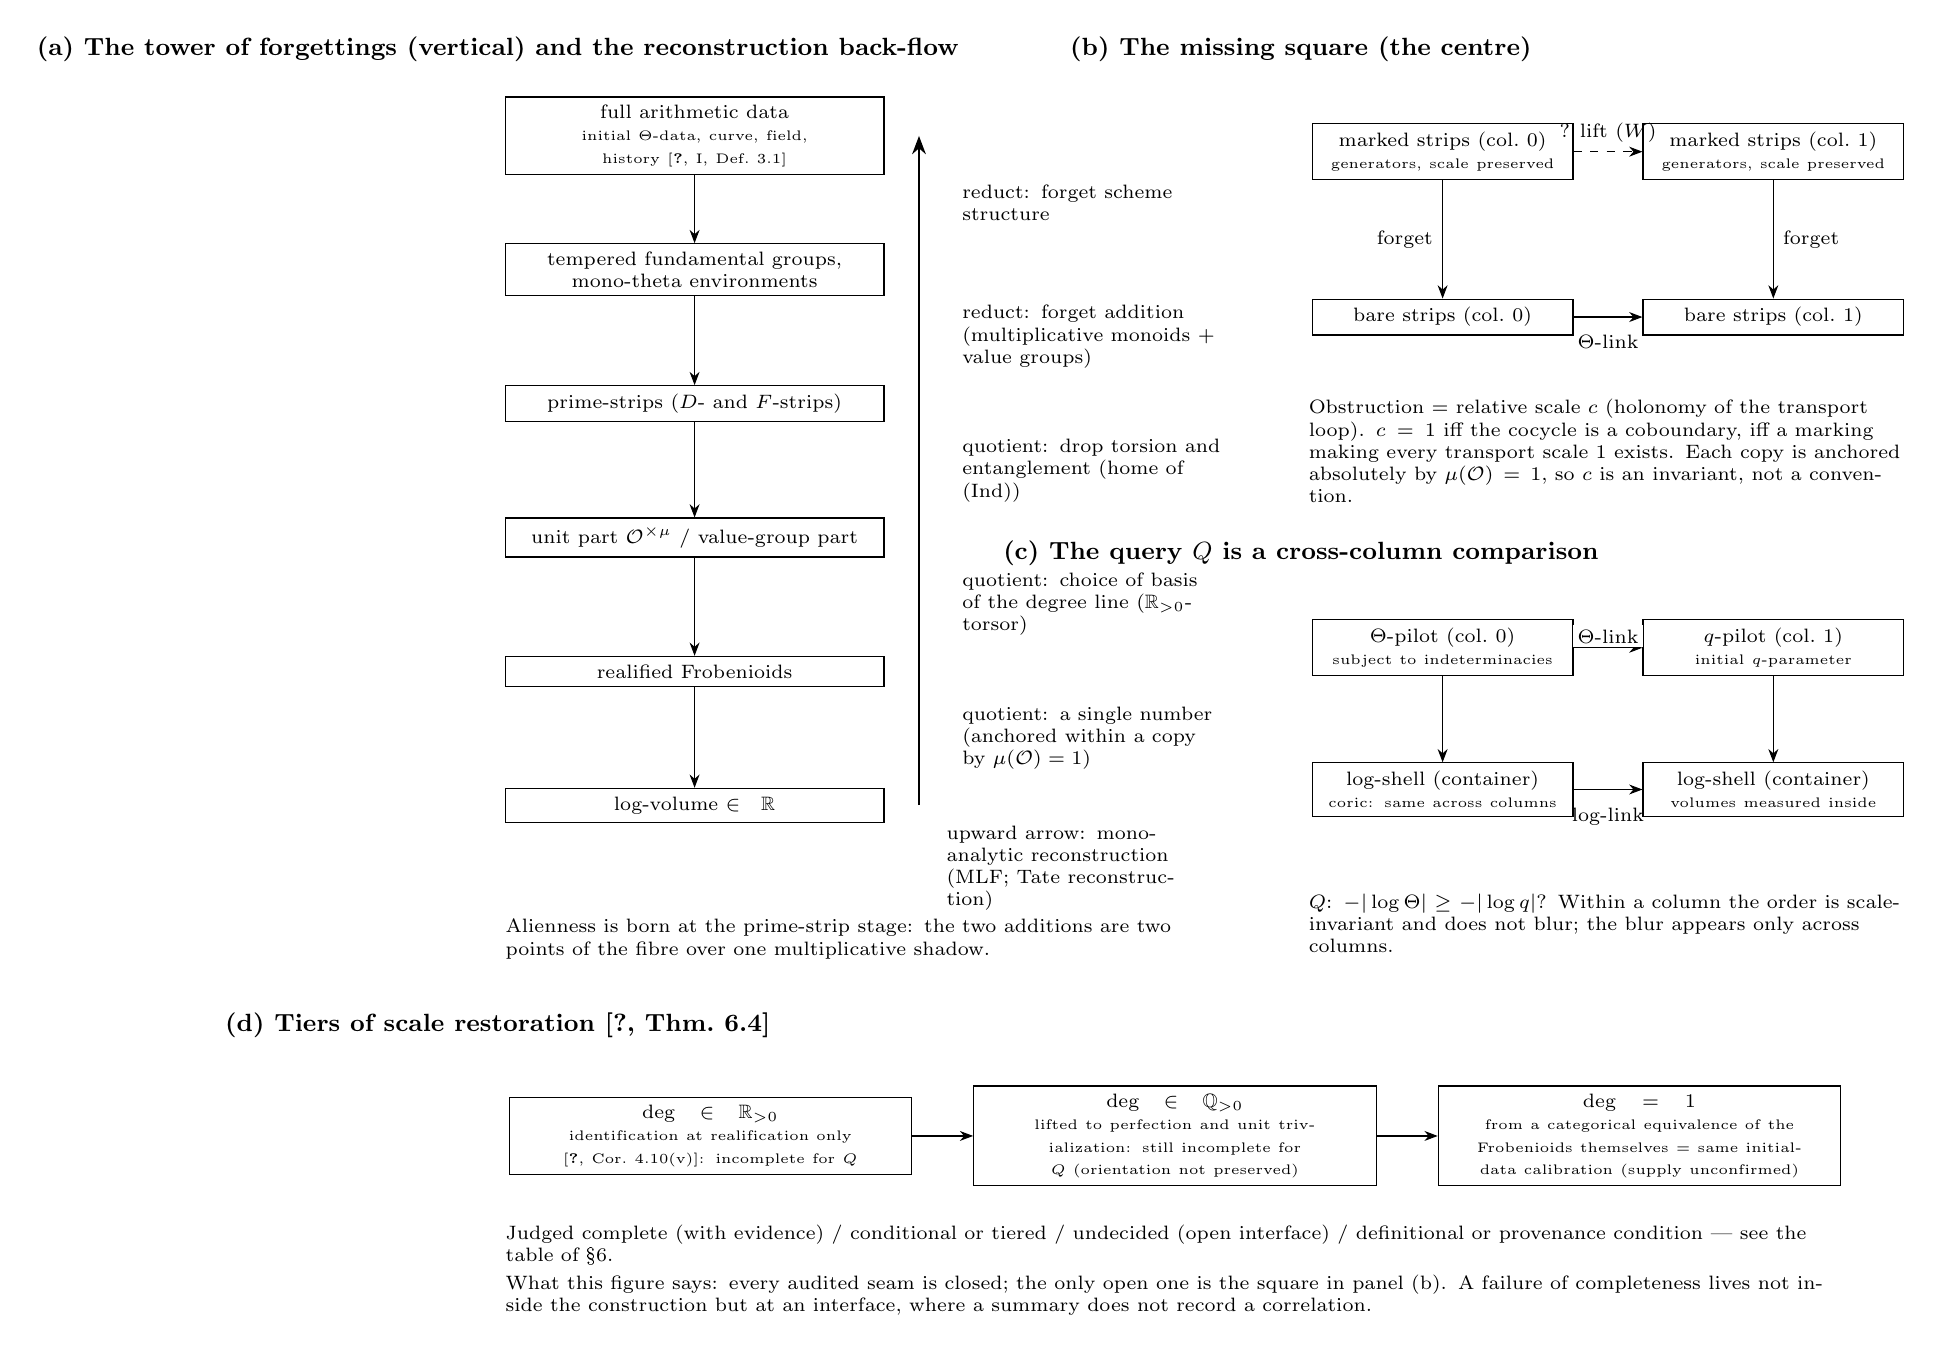
\begin{tikzpicture}[>=Stealth,
  box/.style={draw, align=center, font=\scriptsize, inner sep=3pt},
  note/.style={align=left, font=\scriptsize, inner sep=2pt},
  ttl/.style={font=\small\bfseries, align=left}]

% ---------- (a) tower ----------
\node[ttl] at (0,20.3) {(a) The tower of forgettings (vertical)
and the reconstruction back-flow};
\node[box, text width=4.6cm] (a1) at (2.5,19.2)
{full arithmetic data\\ \tiny initial $\Theta$-data, curve, field,
history \cite[I, Def.~3.1]{IUT1}};
\node[box, text width=4.6cm] (a2) at (2.5,17.5)
{tempered fundamental groups,\\ mono-theta environments};
\node[box, text width=4.6cm] (a3) at (2.5,15.8)
{prime-strips ($D$- and $F$-strips)};
\node[box, text width=4.6cm] (a4) at (2.5,14.1)
{unit part $\cO^{\times\mu}$ / value-group part};
\node[box, text width=4.6cm] (a5) at (2.5,12.4)
{realified Frobenioids};
\node[box, text width=4.6cm] (a6) at (2.5,10.7)
{log-volume $\in\mathbb R$};
\draw[->] (a1)--(a2); \draw[->] (a2)--(a3); \draw[->] (a3)--(a4);
\draw[->] (a4)--(a5); \draw[->] (a5)--(a6);
\node[note, text width=3.3cm] at (7.55,18.35)
{reduct: forget scheme structure};
\node[note, text width=3.3cm] at (7.55,16.65)
{reduct: forget addition\\ (multiplicative monoids + value groups)};
\node[note, text width=3.3cm] at (7.55,14.95)
{quotient: drop torsion and entanglement (home of (Ind))};
\node[note, text width=3.3cm] at (7.55,13.25)
{quotient: choice of basis of the degree line
($\mathbb R_{>0}$-torsor)};
\node[note, text width=3.3cm] at (7.55,11.55)
{quotient: a single number (anchored within a copy by
$\mu(\cO)=1$)};
\draw[->, thick] (5.35,10.7) -- (5.35,19.2);
\node[note, text width=3.2cm] at (7.3,9.9)
{upward arrow: mono-analytic reconstruction (MLF; Tate
reconstruction)};
\node[note, text width=8.6cm] at (4.4,9.0)
{Alienness is born at the prime-strip stage: the two additions are
two points of the fibre over one multiplicative shadow.};

% ---------- (b) missing square ----------
\node[ttl] at (10.2,20.3) {(b) The missing square (the centre)};
\node[box, text width=3.1cm] (b1) at (12.0,19.0)
{marked strips (col.~0)\\ \tiny generators, scale preserved};
\node[box, text width=3.1cm] (b2) at (16.2,19.0)
{marked strips (col.~1)\\ \tiny generators, scale preserved};
\node[box, text width=3.1cm] (b3) at (12.0,16.9)
{bare strips (col.~0)};
\node[box, text width=3.1cm] (b4) at (16.2,16.9)
{bare strips (col.~1)};
\draw[->, dashed] (b1)-- node[above, font=\scriptsize]
{? lift ($W$)} (b2);
\draw[->] (b1)-- node[left, font=\scriptsize]{forget} (b3);
\draw[->] (b2)-- node[right, font=\scriptsize]{forget} (b4);
\draw[->] (b3)-- node[below=3pt, font=\scriptsize, align=center,
text width=3.4cm]
{$\Theta$-link} (b4);
\node[note, text width=7.6cm] at (14.1,15.2)
{Obstruction $=$ relative scale $c$ (holonomy of the transport
loop). $c=1$ iff the cocycle is a coboundary, iff a marking making
every transport scale $1$ exists. Each copy is anchored absolutely
by $\mu(\cO)=1$, so $c$ is an invariant, not a convention.};

% ---------- (c) query Q ----------
\node[ttl] at (10.2,13.9) {(c) The query $Q$ is a cross-column
comparison};
\node[box, text width=3.1cm] (c1) at (12.0,12.7)
{$\Theta$-pilot (col.~0)\\ \tiny subject to indeterminacies};
\node[box, text width=3.1cm] (c2) at (16.2,12.7)
{$q$-pilot (col.~1)\\ \tiny initial $q$-parameter};
\node[box, text width=3.1cm] (c3) at (12.0,10.9)
{log-shell (container)\\ \tiny coric: same across columns};
\node[box, text width=3.1cm] (c4) at (16.2,10.9)
{log-shell (container)\\ \tiny volumes measured inside};
\draw[->] (c1)-- node[above, font=\scriptsize, fill=white,
inner sep=1.5pt]{$\Theta$-link} (c2);
\draw[->] (c1)--(c3); \draw[->] (c2)--(c4);
\draw[->] (c3)-- node[below=3pt, font=\scriptsize, align=center,
text width=3.2cm]
{log-link} (c4);
\node[note, text width=7.6cm] at (14.1,9.2)
{$Q$: $-|\log\Theta|\ge-|\log q|$? Within a column the order is
scale-invariant and does not blur; the blur appears only across
columns.};

% ---------- (d) trichotomy ----------
\node[ttl] at (0,7.9) {(d) Tiers of scale restoration
\cite[Thm.~6.4]{FrdI}};
\node[box, text width=4.9cm] (d1) at (2.7,6.5)
{$\deg\in\mathbb R_{>0}$\\ \tiny identification at realification
only \cite[Cor.~4.10(v)]{IUT2}: incomplete for $Q$};
\node[box, text width=4.9cm] (d2) at (8.6,6.5)
{$\deg\in\mathbb Q_{>0}$\\ \tiny lifted to perfection and unit
trivialization: still incomplete for $Q$ (orientation not
preserved)};
\node[box, text width=4.9cm] (d3) at (14.5,6.5)
{$\deg=1$\\ \tiny from a categorical equivalence of the Frobenioids
themselves $=$ same initial-data calibration (supply unconfirmed)};
\draw[->] (d1)--(d2); \draw[->] (d2)--(d3);

% ---------- legend ----------
\node[note, text width=17cm] at (8.6,4.8)
{Judged complete (with evidence) / conditional or tiered /
undecided (open interface) / definitional or provenance condition
--- see the table of \S6.\\[2pt]
What this figure says: every audited seam is closed; the only open
one is the square in panel (b). A failure of completeness lives not
inside the construction but at an interface, where a summary does
not record a correlation.};
\end{tikzpicture}}
\caption{The whole diagram of forgetting and completeness.
(a) The vertical tower of forgettings and the reverse
mono-analytic reconstruction flow. (b) The missing square: the
lower $\Theta$-link arrow exists by \cite[Def.~3.8(ii)]{IUT3}; the
dashed lift to marked prime-strips is the centre of this paper.
(c) The query $Q$ of Corollary~3.12 as a cross-column comparison
inside a common container. (d) The three tiers of
\cite[Thm.~6.4]{FrdI}; the conclusion needs the $\deg=1$ tier.}
\label{fig:whole}
\end{figure}

\clearpage

\begin{thebibliography}{AbsTopIII}

\bibitem[CC77]{CC77} P.~Cousot and R.~Cousot, Abstract
interpretation: a unified lattice model for static analysis of
programs by construction or approximation of fixpoints,
\emph{Proceedings of the 4th ACM SIGACT-SIGPLAN Symposium on
Principles of Programming Languages (POPL~1977)}, ACM, 1977,
238--252.
DOI \href{https://doi.org/10.1145/512950.512973}{10.1145/512950.512973}.

\bibitem[CC79]{CC79} P.~Cousot and R.~Cousot, Systematic design of
program analysis frameworks, \emph{Proceedings of the 6th ACM
SIGACT-SIGPLAN Symposium on Principles of Programming Languages
(POPL~1979)}, ACM, 1979, 269--282.
DOI \href{https://doi.org/10.1145/567752.567778}{10.1145/567752.567778}.

\bibitem[GR97]{GR97} R.~Giacobazzi and F.~Ranzato, Completeness in
abstract interpretation: a domain perspective, in \emph{Algebraic
Methodology and Software Technology (AMAST~1997)}, Lecture Notes in
Computer Science, Springer, Berlin, 1997, 231--245.
DOI \href{https://doi.org/10.1007/BFb0000474}{10.1007/BFb0000474}.

\bibitem[GRS00]{GRS00} R.~Giacobazzi, F.~Ranzato and F.~Scozzari,
Making abstract interpretations complete, \emph{Journal of the ACM}
\textbf{47} (2000), no.~2, 361--416.
DOI \href{https://doi.org/10.1145/333979.333989}{10.1145/333979.333989}.

\bibitem[Moore]{Moore} R.~E.~Moore, \emph{Interval Analysis},
Prentice-Hall, Englewood Cliffs, NJ, 1966.

\bibitem[MKC09]{MKC09} R.~E.~Moore, R.~B.~Kearfott and
M.~J.~Cloud, \emph{Introduction to Interval Analysis}, Society for
Industrial and Applied Mathematics, Philadelphia, 2009.
ISBN 978-0-898716-69-6.

\bibitem[SF97]{FigStolfi} J.~Stolfi and L.~H.~de Figueiredo,
\emph{Self-Validated Numerical Methods and Applications}, monograph
for the 21st Brazilian Mathematics Colloquium, IMPA, Rio de
Janeiro, 1997.

\bibitem[IUT1]{IUT1} S.~Mochizuki, Inter-universal Teichm\"uller
theory I: construction of Hodge theaters, \emph{Publications of the
Research Institute for Mathematical Sciences} \textbf{57} (2021),
no.~1/2, 3--207.
DOI \href{https://doi.org/10.4171/PRIMS/57-1-1}{10.4171/PRIMS/57-1-1}.

\bibitem[IUT2]{IUT2} S.~Mochizuki, Inter-universal Teichm\"uller
theory II: Hodge--Arakelov-theoretic evaluation, \emph{Publications
of the Research Institute for Mathematical Sciences} \textbf{57}
(2021), no.~1/2, 209--401.
DOI \href{https://doi.org/10.4171/PRIMS/57-1-2}{10.4171/PRIMS/57-1-2}.

\bibitem[IUT3]{IUT3} S.~Mochizuki, Inter-universal Teichm\"uller
theory III: canonical splittings of the log-theta-lattice,
\emph{Publications of the Research Institute for Mathematical
Sciences} \textbf{57} (2021), no.~1/2, 403--626.
DOI \href{https://doi.org/10.4171/PRIMS/57-1-3}{10.4171/PRIMS/57-1-3}.

\bibitem[IUT4]{IUT4} S.~Mochizuki, Inter-universal Teichm\"uller
theory IV: log-volume computations and set-theoretic foundations,
\emph{Publications of the Research Institute for Mathematical
Sciences} \textbf{57} (2021), no.~1/2, 627--723.
DOI \href{https://doi.org/10.4171/PRIMS/57-1-4}{10.4171/PRIMS/57-1-4}.

\bibitem[FrdI]{FrdI} S.~Mochizuki, The geometry of Frobenioids I:
the general theory, \emph{Kyushu Journal of Mathematics}
\textbf{62} (2008), no.~2, 293--400.
DOI \href{https://doi.org/10.2206/kyushujm.62.293}{10.2206/kyushujm.62.293}.

\bibitem[EtTh]{EtTh} S.~Mochizuki, The \'etale theta function and
its Frobenioid-theoretic manifestations, \emph{Publications of the
Research Institute for Mathematical Sciences} \textbf{45} (2009),
no.~1, 227--349.
DOI \href{https://doi.org/10.2977/prims/1234361159}{10.2977/prims/1234361159}.

\bibitem[AbsTopIII]{AbsTopIII} S.~Mochizuki, Topics in absolute
anabelian geometry III: global reconstruction algorithms,
\emph{Journal of Mathematical Sciences, the University of Tokyo}
\textbf{22} (2015), no.~4, 939--1156.

\bibitem[SS18]{SS18} P.~Scholze and J.~Stix, Why \emph{abc} is
still a conjecture, report, 14 May 2018.
Available at
\url{https://www.math.uni-bonn.de/people/scholze/WhyABCisStillaConjecture.pdf}.

\bibitem[LANA]{LANA} Project LANA, \emph{Project LANA interim
report on IUT theory}, July 2026, 50~pp.

\bibitem[lana]{lana} Project LANA, \emph{lana-agents/iut} (Lean
repository), \url{https://github.com/lana-agents/iut}.  File
\texttt{Iut/WallEquiv/NonDerivable.lean}, referenced at commit
553076a (3 November 2026).

\bibitem[U26]{U26} T.~Urahigashi, Where Theorem~3.11 sits: the
log-volume content of the results cited in the proof of IUT~III,
Corollary~3.12, does not imply its conclusion, version 1.2.1,
Zenodo, 2026.
DOI \href{https://doi.org/10.5281/zenodo.24104932}{10.5281/zenodo.24104932}.

\bibitem[UCS]{UCS} T.~Urahigashi, Two computations of the height
inequality and the multiradial algorithm: reading IUT from the
viewpoint of computer science, Zenodo, 2026.
DOI \href{https://doi.org/10.5281/zenodo.24039369}{10.5281/zenodo.24039369}.

\bibitem[UHoTTa]{UHoTTa} T.~Urahigashi, Segment or loop? A
homotopy-type-theoretic overview of the dispute over
Corollary~3.12 of inter-universal Teichm\"uller theory, Zenodo,
2026.
DOI \href{https://doi.org/10.5281/zenodo.24039360}{10.5281/zenodo.24039360}.

\bibitem[UHoTTb]{UHoTTb} T.~Urahigashi, Reading the IUT dispute
through indexed identifications: an educational model in
undergraduate mathematics, Zenodo, 2026.
DOI \href{https://doi.org/10.5281/zenodo.24039367}{10.5281/zenodo.24039367}.

\end{thebibliography}

\end{document}
